\documentclass[11pt,graphicx,caption,rotating]{article}
\textheight=24cm
\textwidth=18cm
\topmargin=-2cm
\oddsidemargin=0cm
\usepackage[utf8x]{inputenc}
\usepackage[activeacute,spanish]{babel}
\usepackage{amssymb,amsfonts}
\usepackage[tbtags]{amsmath}
\usepackage{lscape}
\usepackage{pict2e}
\usepackage{float}
\usepackage[all]{xy}
\usepackage{graphics,graphicx,color,colortbl}
\usepackage{times}
\usepackage{subfigure}
\usepackage{wrapfig}
\usepackage{multicol}
\usepackage{cite}
\usepackage{url}
\usepackage[tbtags]{amsmath}
\usepackage{amsmath,amssymb,amsfonts,amsbsy}
\usepackage{bm}
%\usepackage{algorithm}
%\usepackage{algorithmic}
\usepackage[centerlast, small]{caption}
\usepackage[colorlinks=true, citecolor=blue, linkcolor=blue, urlcolor=blue,breaklinks=true]{hyperref}

\begin{document}
\begin{landscape}
\begin{figure}[H]
	\centering
		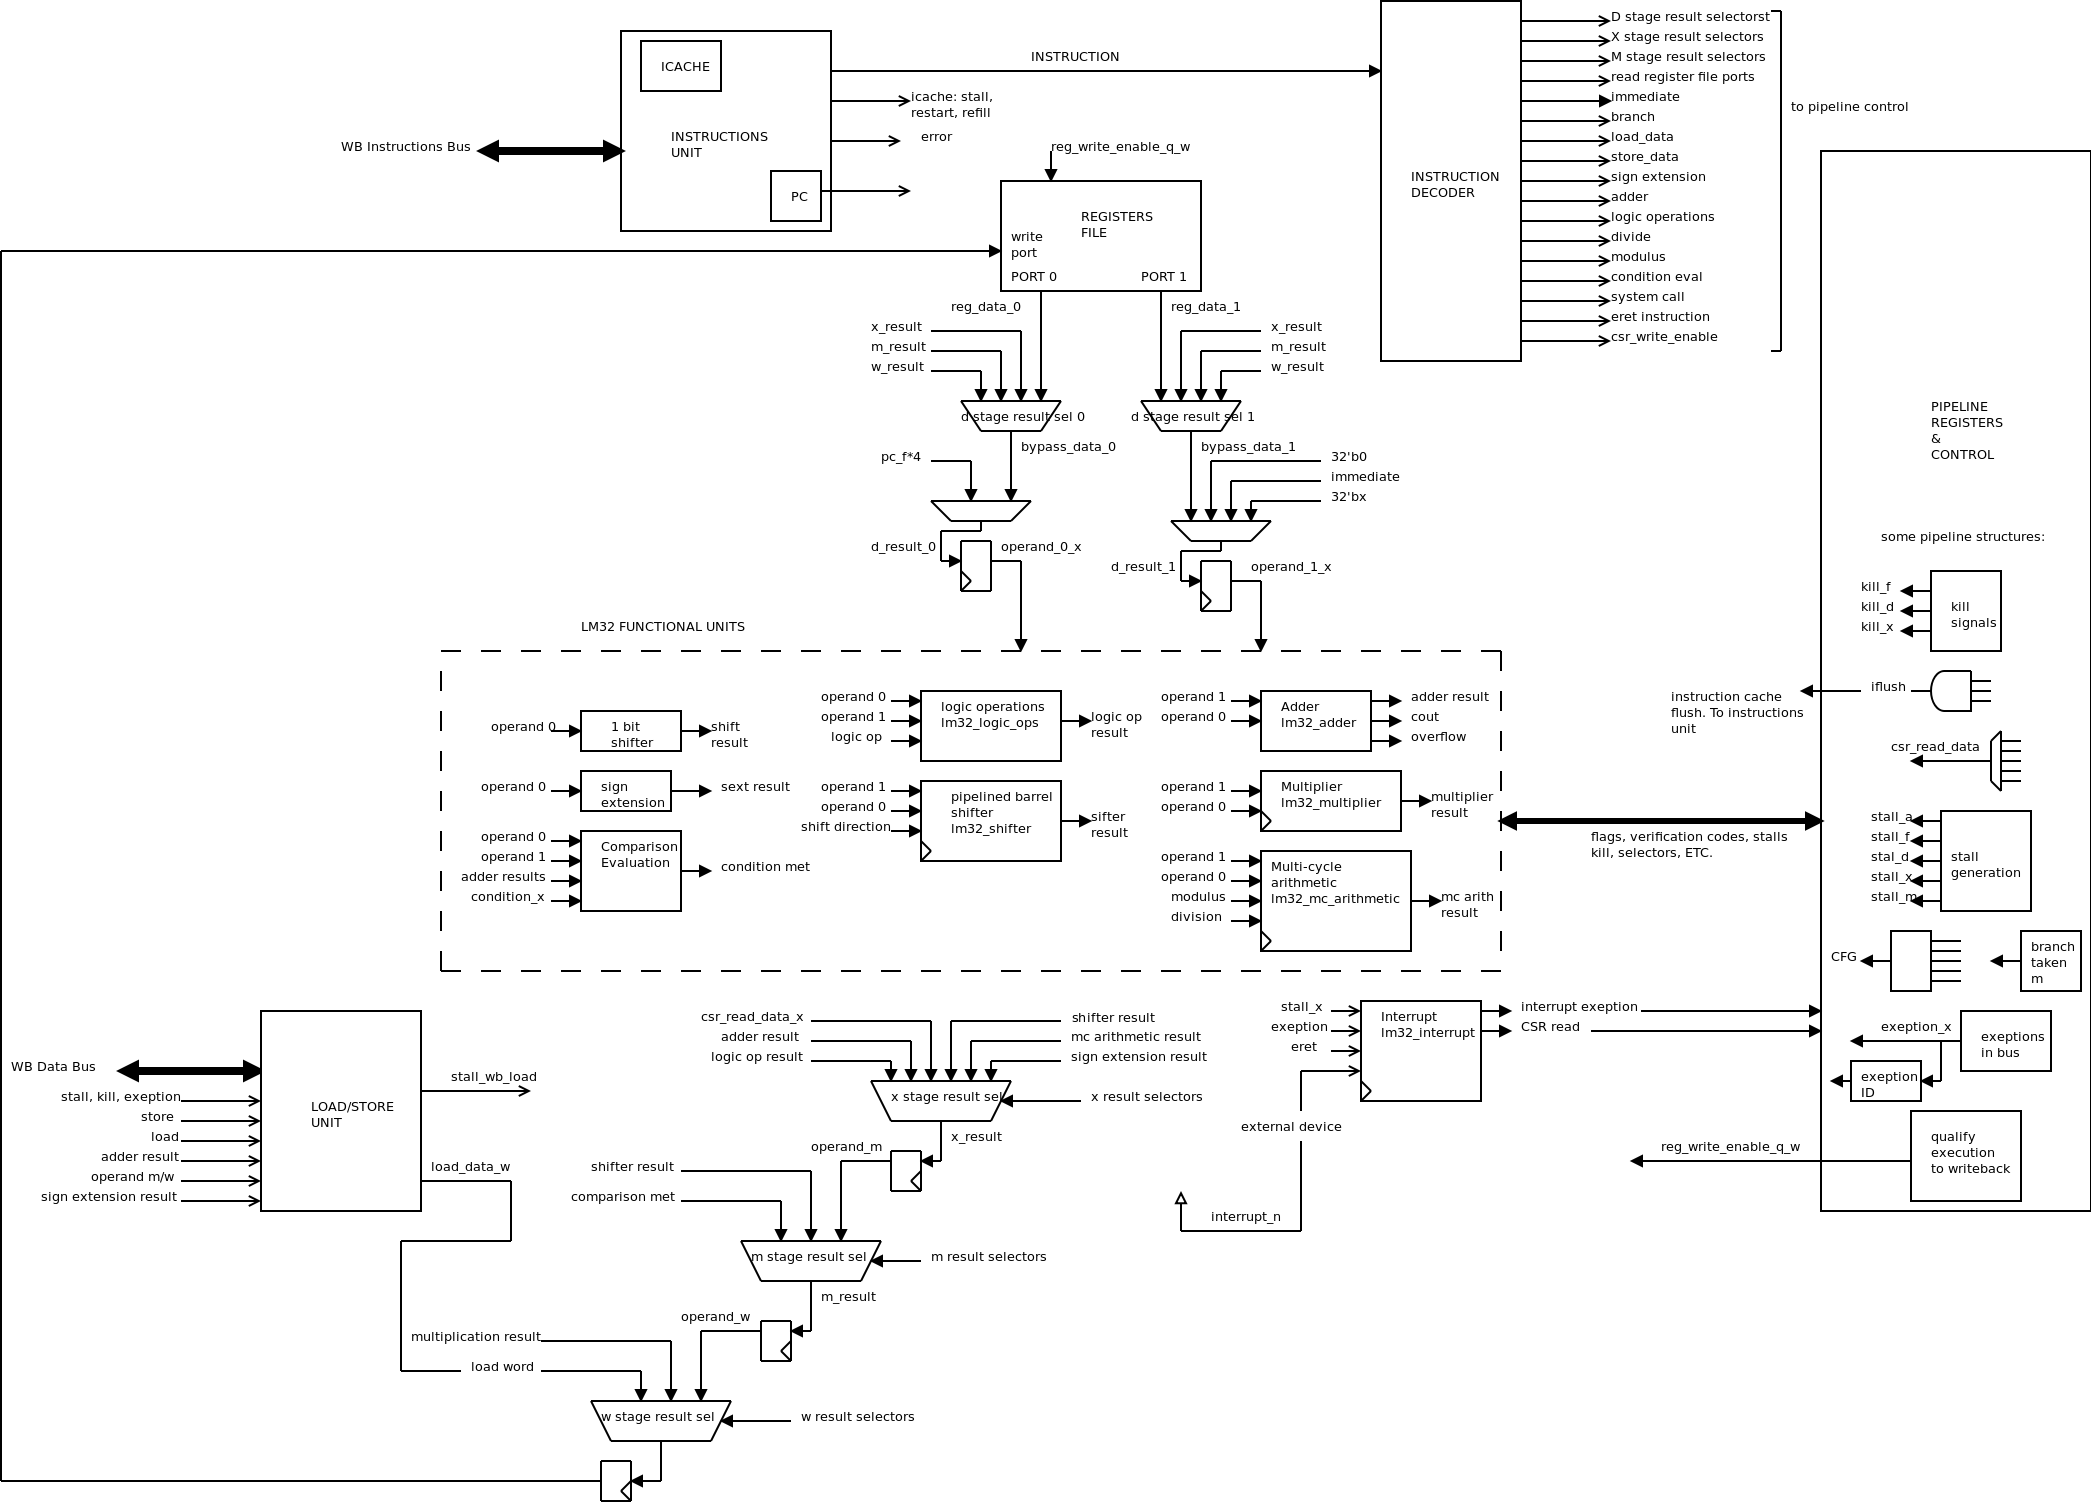
\includegraphics[scale=0.32]{DATAPATH.png}
	\caption{Diagrama completo para el datapath.}
	\label{fig2}
\end{figure}
\begin{figure}[H]
	\centering
		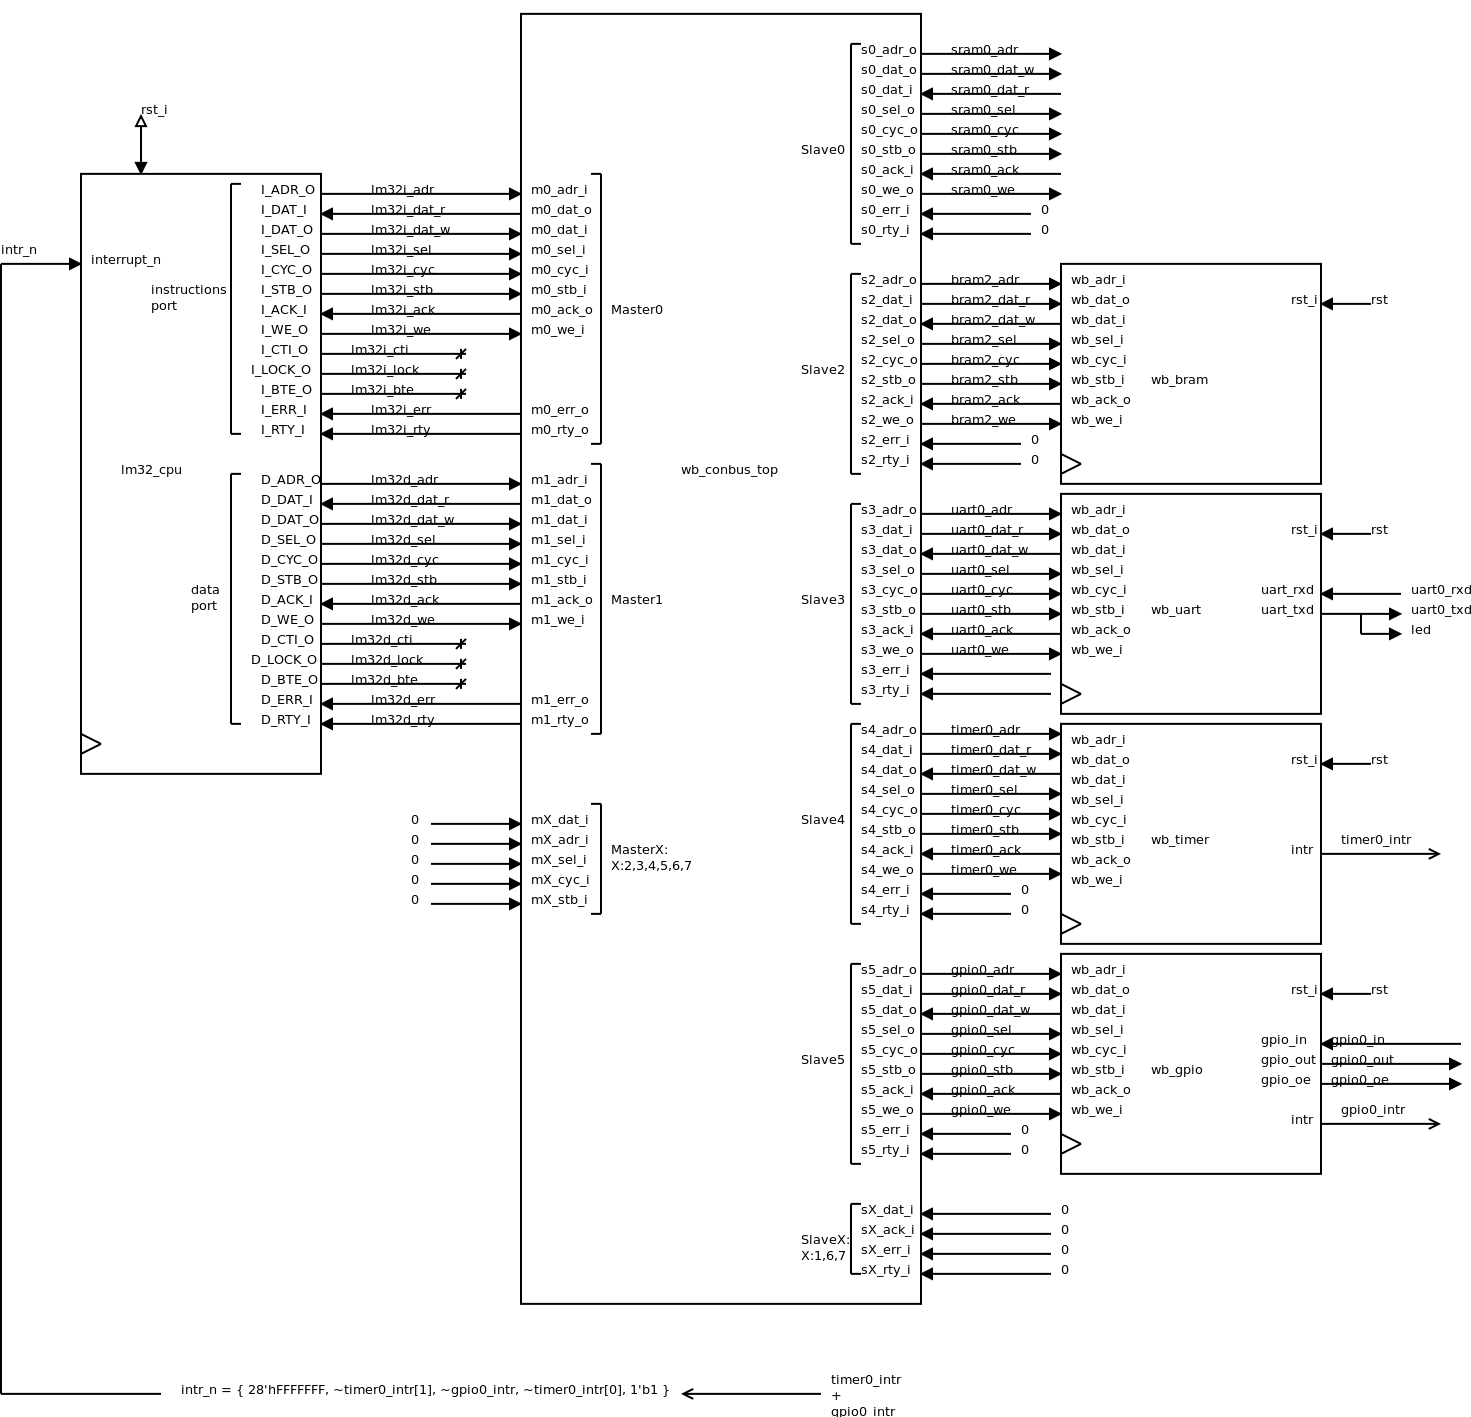
\includegraphics[scale=0.32]{system_v2.png}
	\caption{Diagrama completo para el datapath.}
	\label{fig3}
\end{figure}
\end{landscape}
\end{document}
